\documentclass[options]{article}
\usepackage[]{url}
\usepackage{graphicx}
\usepackage{hyperref}
\usepackage{mathtools}

\begin{document}
\title{Simulation of two interacting squirmers}
\author{Robin and Justine}
\date{May, 2024}
\maketitle

\section{Context}
Our project is part of the ANR project NEMO, Control of Magnetic Micro-swimmers in Complex and Confined Environments.
Currently, a team of researchers is developing numerical methods to control a micro-swimmer in the arteries
of the human body.\\
The Squirmer model simulates bacteries with cilia by imposing boundary conditions.\\
Ultimately, the goal of these robots is to treat cancer cells.\\

\vspace{0.5cm}
\section{Objectives}
Our goal is to model the dynamics of two interacting squirmer, influenced by hydrodynamic \cite{Brumley} and collision forces.\\
We will start by reformulating the formulas of all present forces and torques.\cite{Brumley}\cite{Lauga}\\
In addition we will implement this model to realize numerical experiments. The aim of these experiments is: 
\begin{itemize}
    \item Investigating the effects of varying the distance between the squirmers to observe
    potential modifications in their behaviors.
    \item To explore the impact of altering the parameter $\beta$, which defines the
    type of squirmers (pusher, puller, neutral), on their interactions.
    \item To conduct a comparative analysis of the interaction between a squirming micro-robot and a 
    boundary. This analysis will involve varying the initial angle of the the micro-robot, the distance between the swimmer and the wall, as well as the parameter $\beta$, 
    to comprehensively understand their influence on the system dynamics.
\end{itemize}

\newpage
\section{Roadmap}
\begin{center}
    \href{https://github.com/orgs/master-csmi/projects/23/views/2}{Roadmap}
    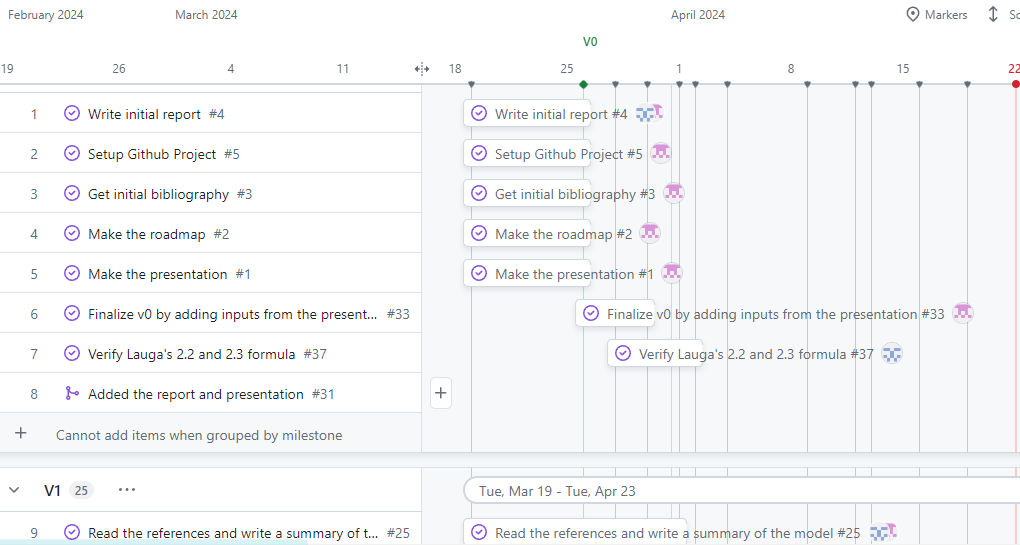
\includegraphics[width=0.9\textwidth]{Presentation/V0/images/roadmapV0_1.png}
    \vspace{1em} % Ajoute un espace vertical
    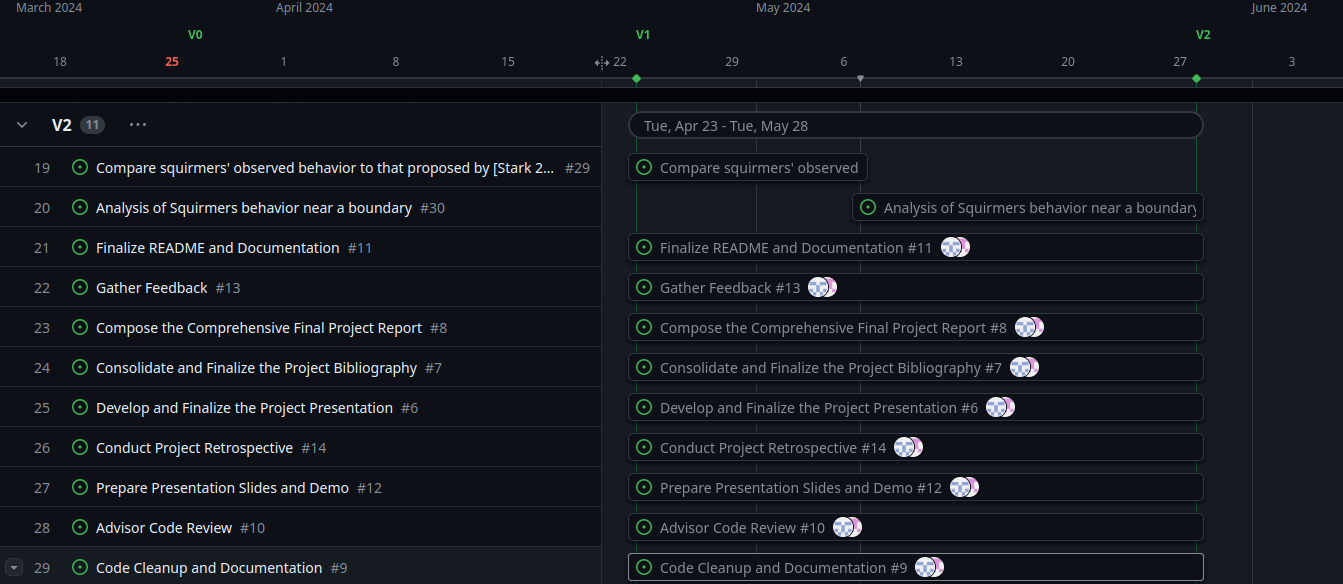
\includegraphics[width=0.9\textwidth]{Presentation/V0/images/roadmapV0_2.png}
\end{center}

\newpage
\section{Equation}
The velocity $u$ is defined like :
\newline $$ \left\{ u_r(R,\theta)=0
\atop u_\theta(R,\theta) = B_1\mathrm{sin}(\theta)+B_2\mathrm{sin}(\theta)\mathrm{cos}(\theta) \right.$$
in polar coordinates.
\\ By asking $\beta=\frac{B_2}{B_1}$, we have :
$u_\theta(R,\theta) = B_1(\mathrm{sin}(\theta) + \beta \mathrm{sin}(\theta)\mathrm{cos}(\theta))$, which $\beta$ is the type of the squirmers :
$$\left\{
    \begin{array}{ll}
        \beta = 0 : \mathrm{neutral} \\
        \beta < 0 : \mathrm{pusher} \\
        \beta > 0 : \mathrm{puller} \\
    \end{array}
\right.$$
\\ Now let us put $u$ in cartesian coordinates :
\begin{align*}
    u &= \begin{pmatrix}
   u_x \\
   u_y
\end{pmatrix}
= \begin{pmatrix}
   \mathrm{cos}(\theta) & -\mathrm{sin}(\theta) \\
   \mathrm{sin}(\theta) & \mathrm{cos}(\theta)
\end{pmatrix}
\begin{pmatrix}
   u_r \\
   u_\theta
\end{pmatrix} \\
&= B_1 (1 + \beta \mathrm{cos}(\theta))
\begin{pmatrix}
   -\mathrm{sin}^2(\theta) \\
   \mathrm{sin}(\theta)\mathrm{cos}(\theta)
\end{pmatrix}
\end{align*}
We have $B_1$ = $\frac{3}{2}u_0$, so :
$u$ = $\frac{3}{2}u_0 (1 + \beta \mathrm{cos}(\theta))
\begin{pmatrix}
   -\mathrm{sin}^2(\theta) \\
   \mathrm{sin}(\theta)\mathrm{cos}(\theta)
\end{pmatrix}$

We pose $e_r$ = $\begin{pmatrix}
   \mathrm{cos}(\theta) \\
   \mathrm{sin}(\theta)
\end{pmatrix}$ the direction of the squirmer at each instant relative to $e$ = 
$\begin{pmatrix}
   \mathrm{cos}(\phi) \\
   \mathrm{sin}(\phi) \end{pmatrix}$ or we fixe $\phi$ = 0, so : $e$ = $\begin{pmatrix}
   1 \\
   0 \end{pmatrix}$.
\\ Also, 
\begin{align*}
u_r &= \frac{3}{2}u_0(1+\beta (e.e_r)) [(e.e_r)e_r - e] \\ 
&= \frac{3}{2}u_0\left(1+\beta \begin{pmatrix}
   1 \\
   0 \end{pmatrix}\begin{pmatrix}
   \mathrm{cos}(\theta) \\
   \mathrm{sin}(\theta)
\end{pmatrix}\right) \left[ \left( \begin{pmatrix}
   1 \\
   0 \end{pmatrix}\begin{pmatrix}
   \mathrm{cos}(\theta) \\
   \mathrm{sin}(\theta)
\end{pmatrix}\right) \begin{pmatrix}
   \mathrm{cos}(\theta) \\
   \mathrm{sin}(\theta)
\end{pmatrix} - \begin{pmatrix}
   1 \\
   0 \end{pmatrix}\right] \\
 &= \frac{3}{2}u_0\left(1+\beta \mathrm{cos}(\theta) \right) \begin{pmatrix}
   \mathrm{cos}^2(\theta)-1 \\
   \mathrm{sin}(\theta)\mathrm{cos}(\theta)
\end{pmatrix} \\
&= \frac{3}{2}u_0\left(1+\beta \mathrm{cos}(\theta) \right) \begin{pmatrix}
   -\mathrm{sin}^2(\theta) \\
   \mathrm{sin}(\theta)\mathrm{cos}(\theta)
\end{pmatrix} 
\end{align*}

\vspace{0.5 cm}
Also, $u$ in cartesian coordinates is like :
\begin{equation*}
\boxed{u_r = \frac{3}{2}u_0(1+\beta (e.e_r)) [(e.e_r)e_r - e]
    = \frac{3}{2}u_0\left(1+\beta \mathrm{cos}(\theta) \right) \begin{pmatrix}
   -\mathrm{sin}^2(\theta) \\
   \mathrm{sin}(\theta)\mathrm{cos}(\theta)
\end{pmatrix}}
\end{equation*}

\nocite{*}
\bibliographystyle{plain}
\bibliography{/bibliography/biblio}
\end{document}